\chapter{Results}\label{sec:results}

This section discusses the results of the case study used to validate the software developed for this project, using 2D and 3D models of an edge crack in a finite plate. The parameters of both the 2D and 3D models were adjusted in order to perform finite element analyses for varying mesh densities, integration domains, weight functions, and crack lengths. The software was then used to export the results of these finite element analyses, and then to calculate the J-integrals and stress intensity factors for each set of parameters. This allowed the impact of these parameters on the results to be understood, and therefore used to demonstrate that the software implemented the equivalent domain integral method correctly. The results obtained via the software were also compared to analytically calculated results to validate that the J-integral and stress intensity factors produced were correct.

\newpage
\section{Mesh Convergence}

A mesh convergence study was conducted in order to find the point at which the results obtained from the finite element analysis became independent of the density of the mesh used. Mesh convergence studies are a common practice when performing finite element analysis, as they allow the competing demands of solution accuracy and computational resources to be balanced in order to obtain sufficiently accurate results as efficiently as possible \cite{hellen_how_2001}. In order to perform the mesh convergence study, the configuration parameter \texttt{crack\_element\_count} was used to vary the size of the elements located close to the crack tip. A function was also created to determine the average element size directly around the crack tip, in order to obtain a more direct measurement of the element size rather than simply using the number of elements.

The mesh convergence study was limited to the area close to the crack tip, since this was the area that was being used to calculate the J-integral. A coarse mesh of 2.5 mm elements was considered sufficient to model the remote areas of the problem, given the simple loading and boundary conditions used. Although a stress value is usually used as the value for comparison, the options for stress in this case were to use a stress value remote from the crack tip, or use the stresses close to the crack tip. The remote stresses were not relevant to the actual solution, while the crack tip stresses were prone to significant variation due to the nature of the crack tip singularity. Therefore, the J-integral was used to measure the mesh sensitivity, as it was the most relevant parameter to the specific problem being analysed. An initial investigation of the results found that the solution maintained domain independence across various configurations (discussed in the following section) -- therefore, the mesh convergence study was conducted using solely the fifth annular domain from the crack tip.

Figure \ref{fig:j_integral_vs_mesh} presents the results of the mesh sensitivity study, by plotting the J-integral against the crack tip element size. Significant deviation was observed in the results between crack tip elements of size 1.5 mm and 0.6 mm. However, the results converged at a crack tip element size of around 0.5 mm. The crack tip element size used for the remainder of the analysis was 0.461 mm, which corresponded to 15 elements along the 10 mm crack (\texttt{crack\_element\_count}), with a bias ratio of 2 (\texttt{crack\_element\_bias}).

\begin{figure}[H]
	\centering
	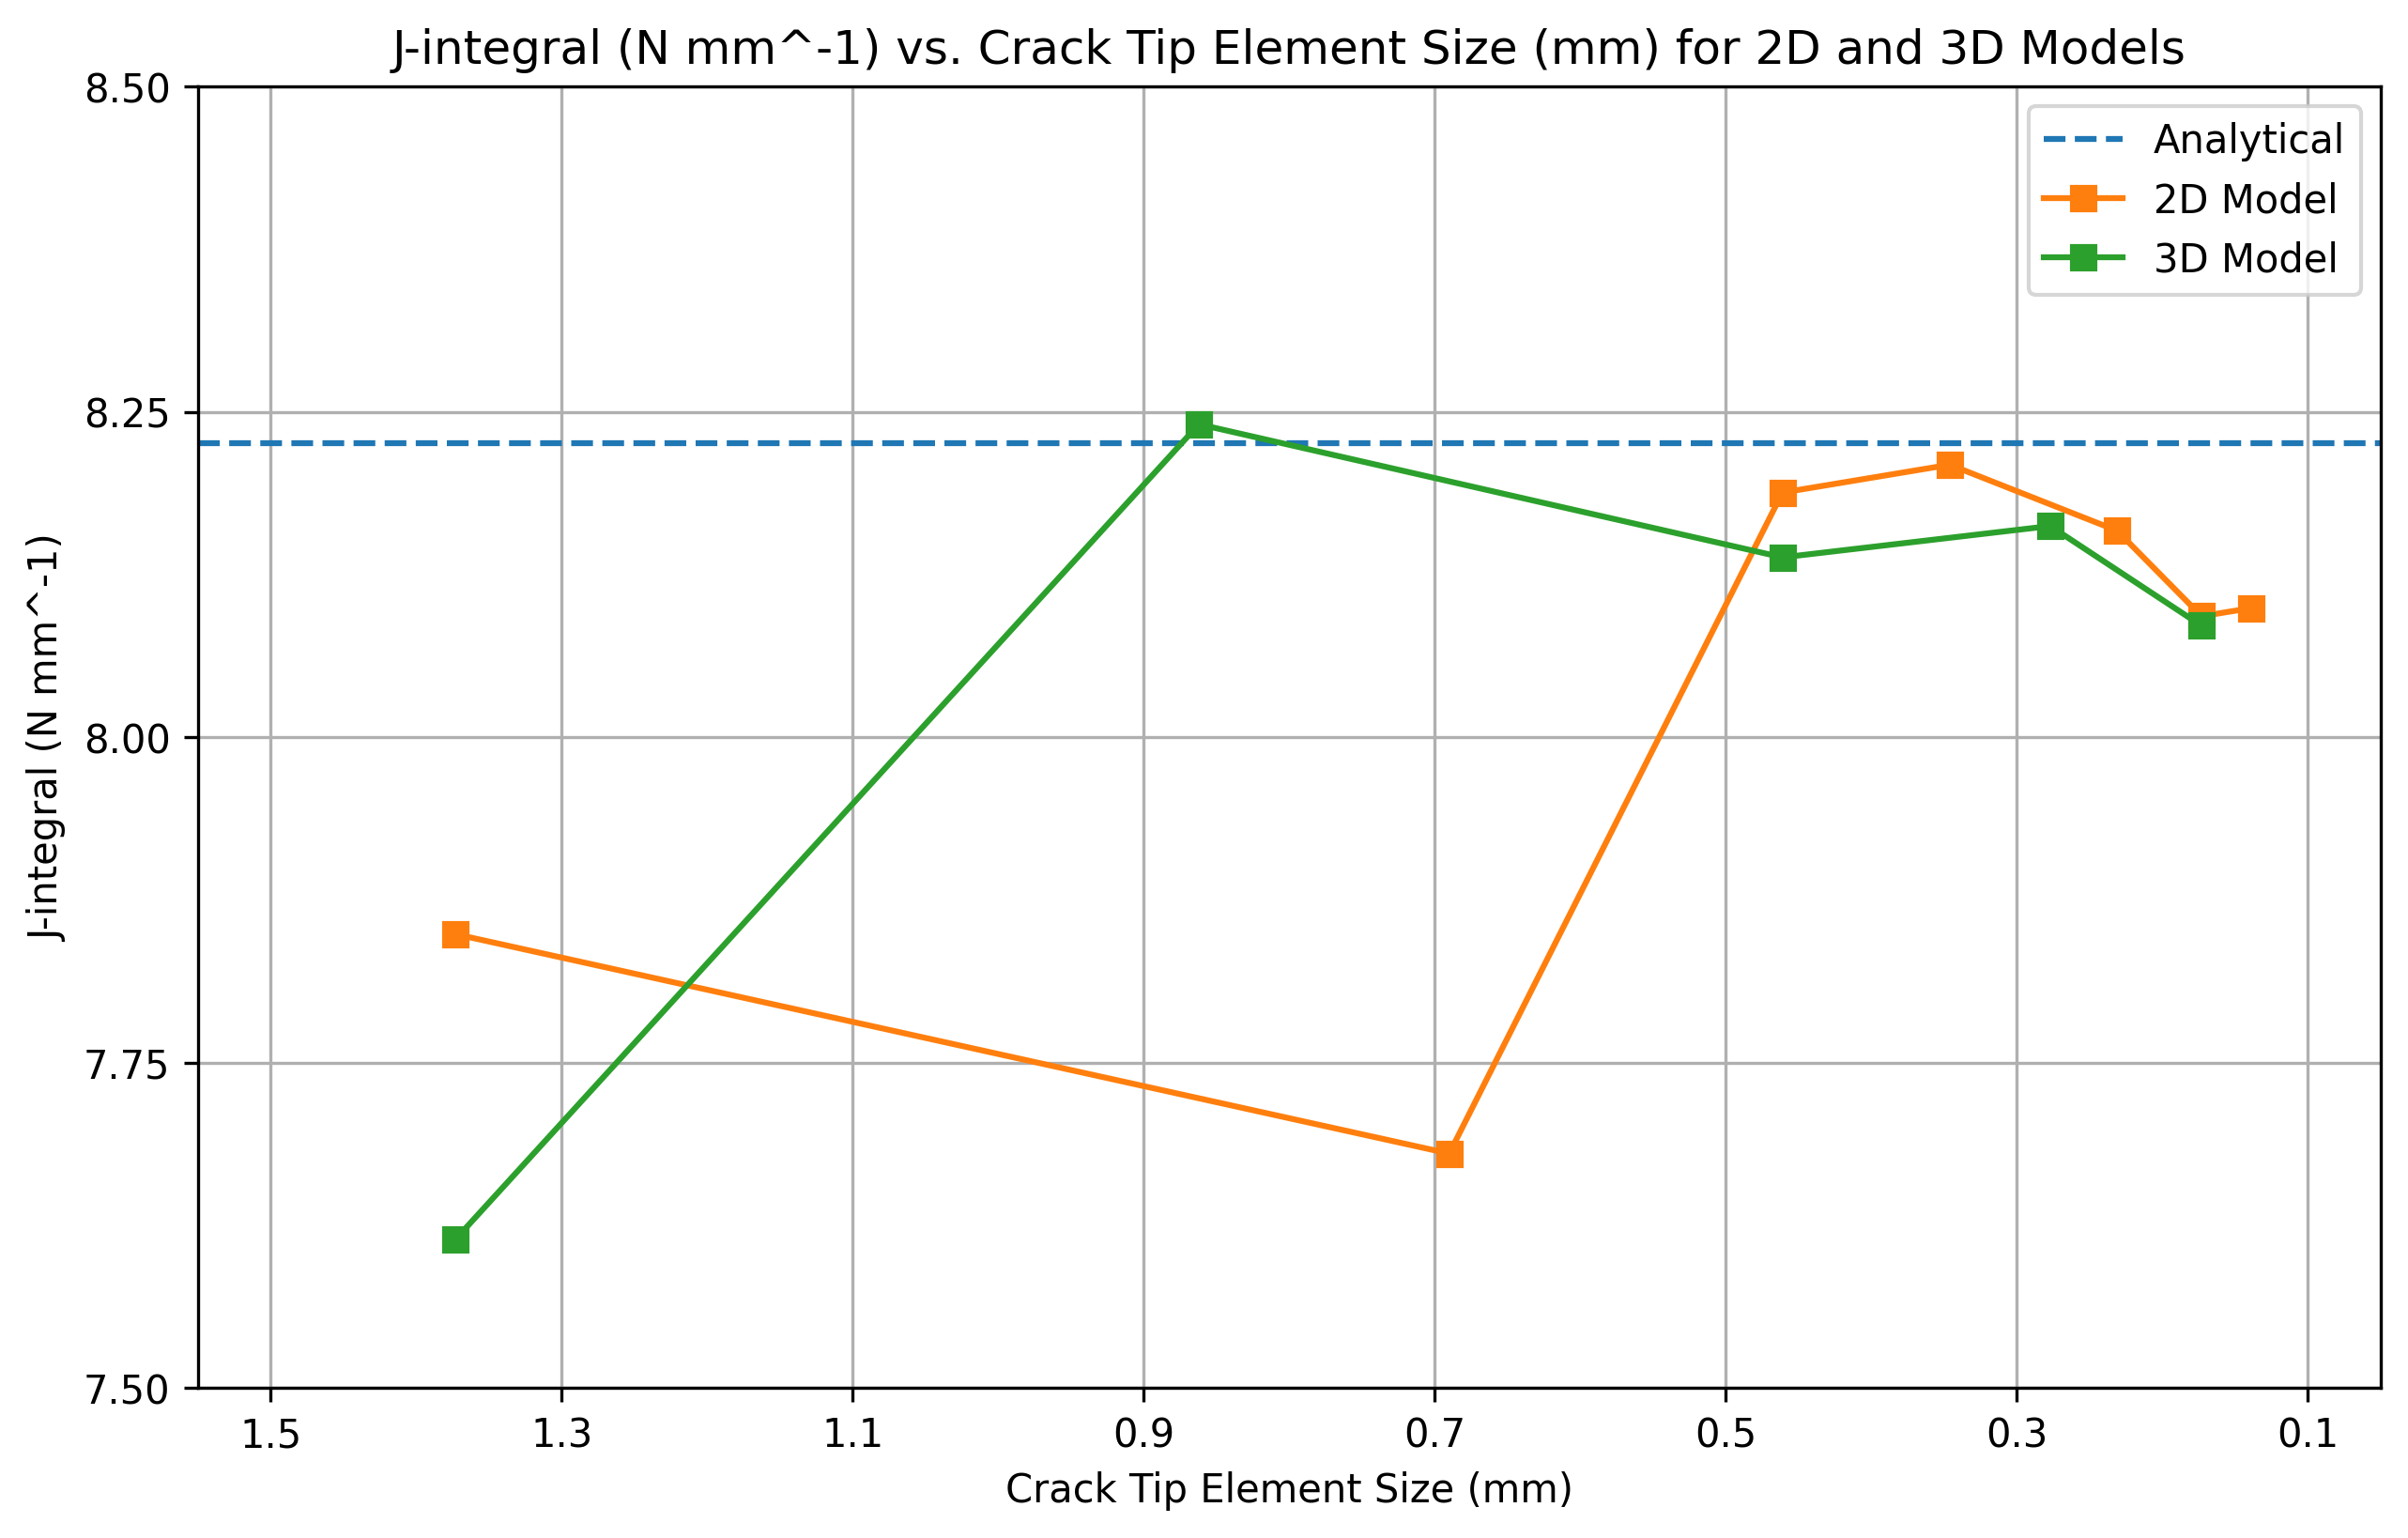
\includegraphics[width=\textwidth]{j_integral_vs_mesh.png}
	\caption{J-integral $(N\ mm^{-1}$ vs crack tip element size (mm) for a $10\ mm$ edge crack).}
	\label{fig:j_integral_vs_mesh}
\end{figure}

\section{Domain Independence}

A key feature of the J-integral is the demonstration of path-independence -- that is, the calculated value should be independent of the path around the crack which was selected. This equally applies to domain selection when using the equivalent domain integral method. Therefore, demonstrating that the J-integral values calculated by the software were domain-independent was critical in order to validate that the method had been implemented correctly.

To accomplish this, the software was implemented such that multiple non-overlapping domains were defined, and a separate J-integral was calculated for each domain (as described in §\ref{sec:implementation_domains}). This allowed the domain independence of the results to be verified by comparing the J-integral results obtained for each domain. The J-integral results for each domain -- for the reference model with a crack length of 10 mm -- were recorded and plotted , along with a analytical value obtained via the analytical expression for the stress intensity factor (Equations \ref{eq:sif} and \ref{eq:beta_edge_crack}). This is presented in Figure \ref{fig:j_integral_vs_domain}.

\begin{figure}[H]
	\centering
	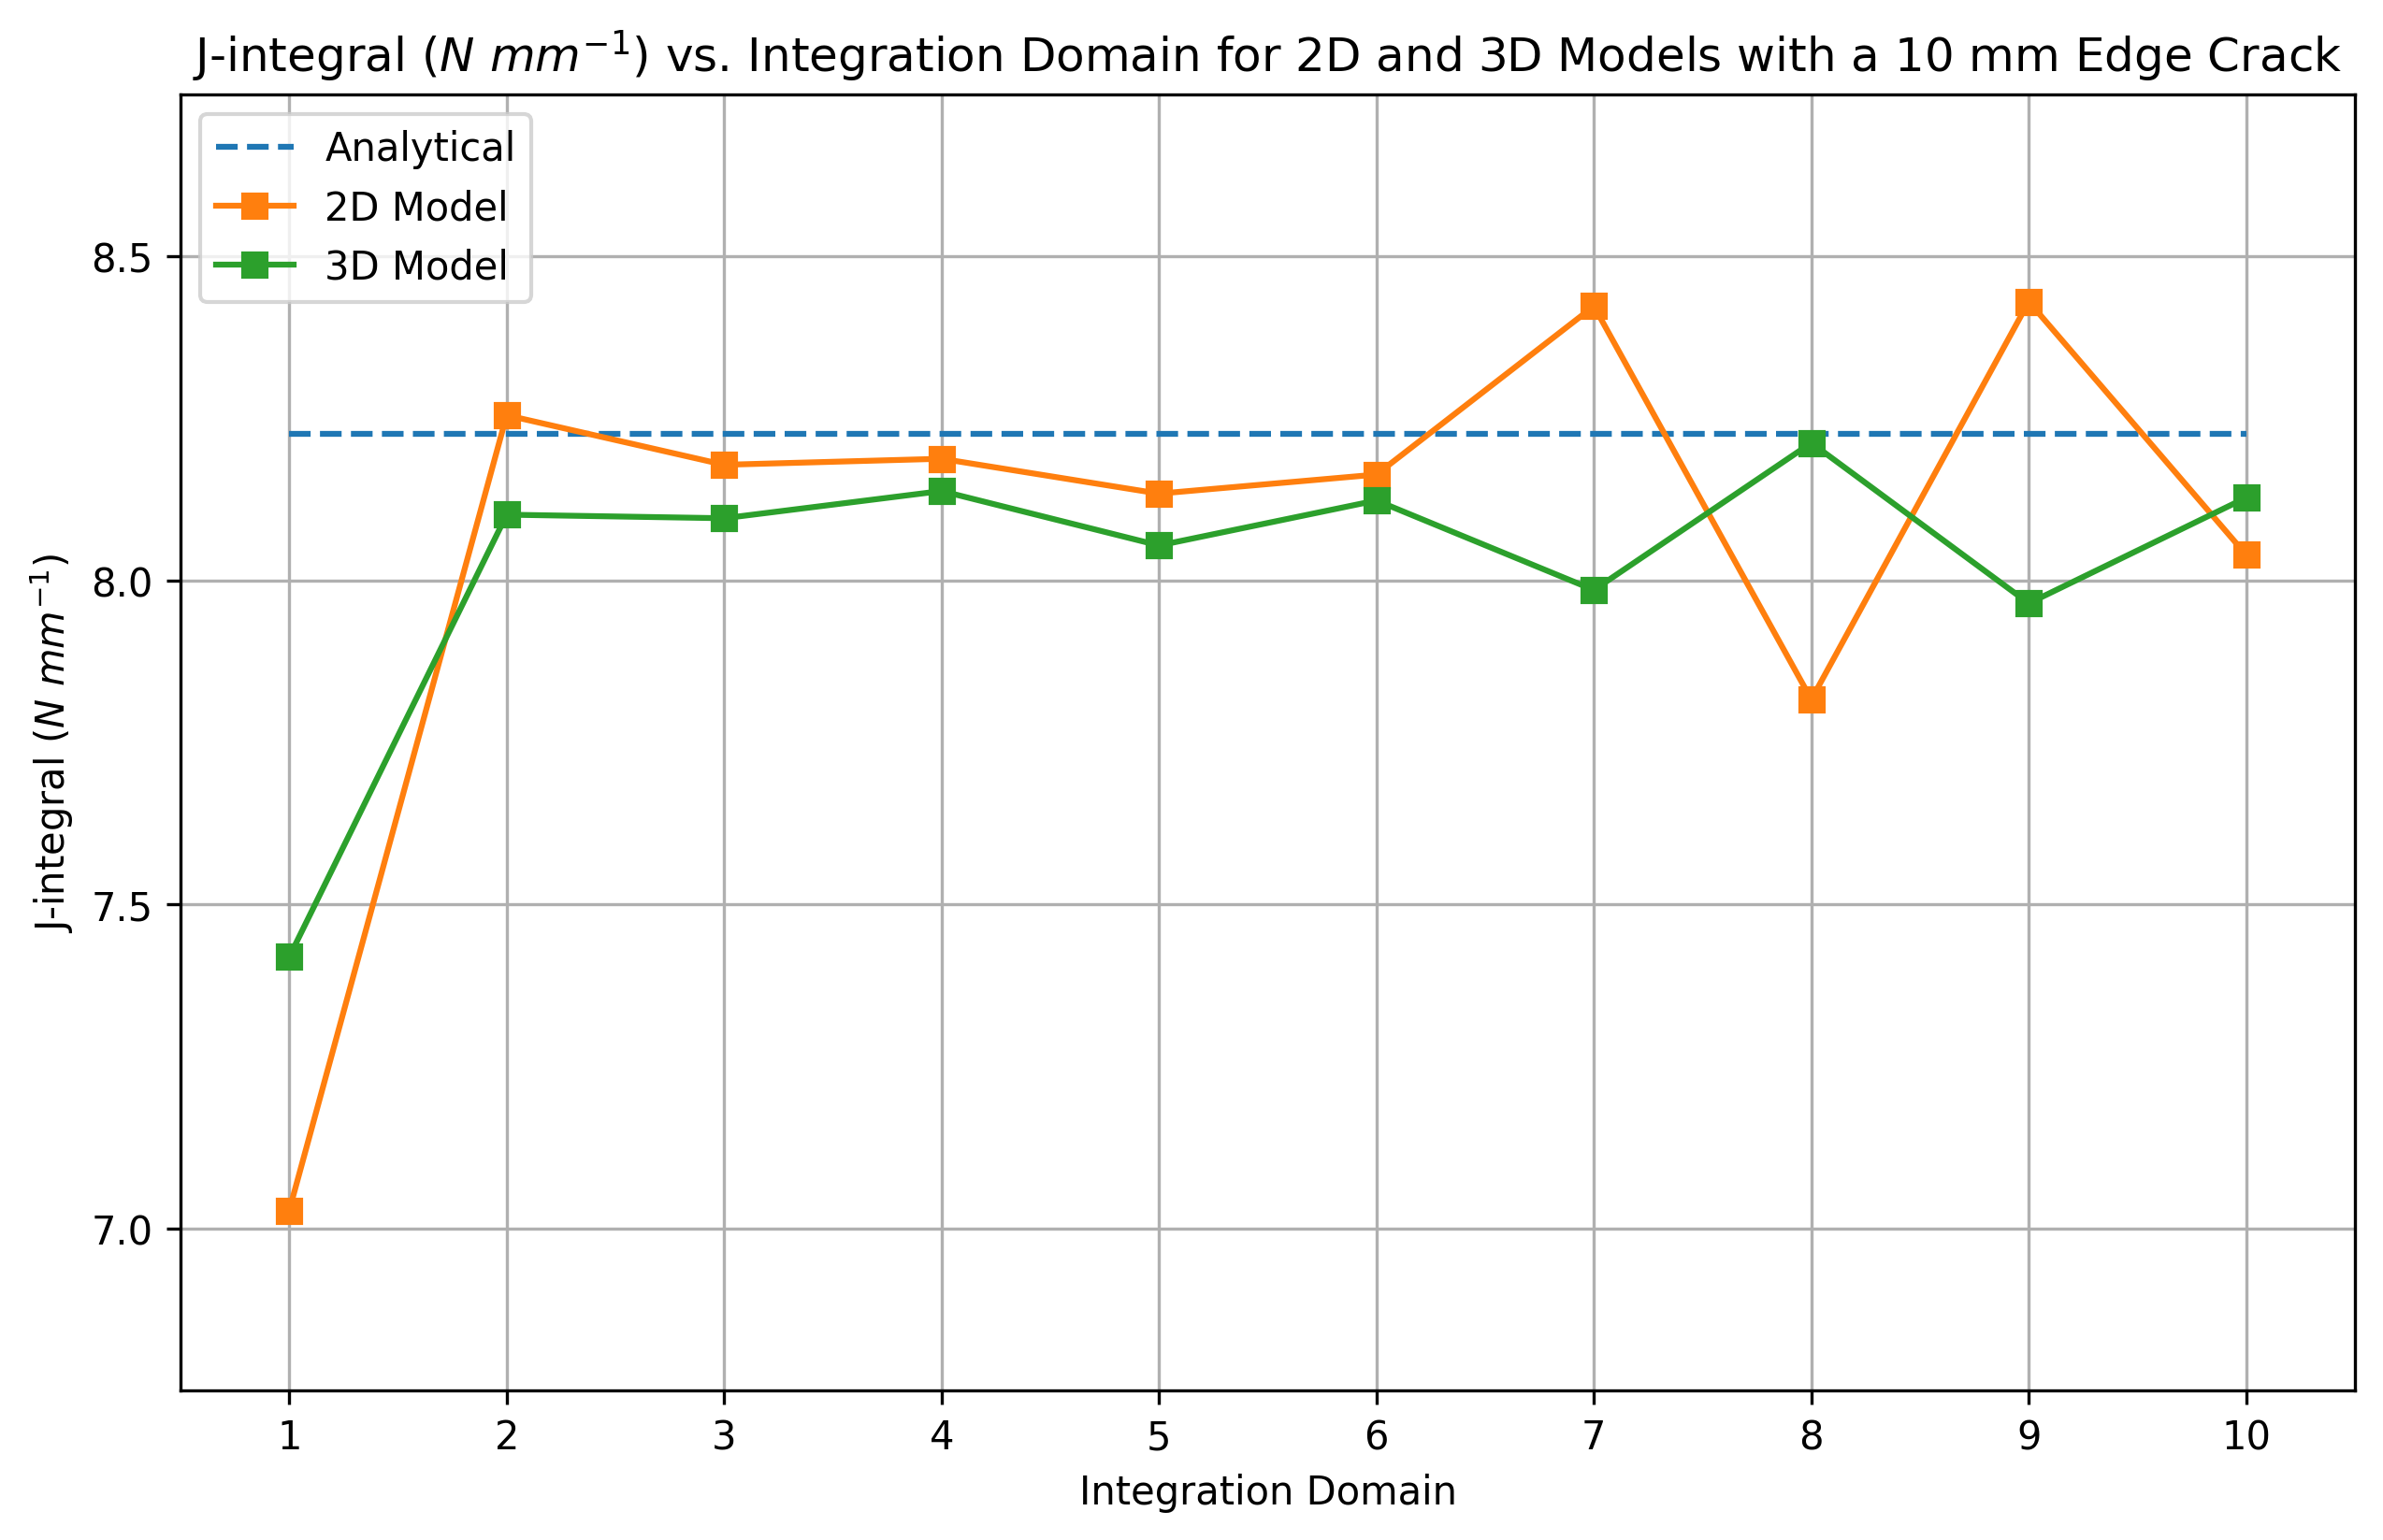
\includegraphics[width=\textwidth]{j_integral_vs_domain.png}
	\caption{J-integral $(N\ mm^{-1}$ vs integration domain for a $10\ mm$ edge crack).}
	\label{fig:j_integral_vs_domain}
\end{figure}

Overall, the J-integral definitively exhibited domain independence beyond the first domain, with maximum deviations of under 2\% from the mean. The J-integral calculated for the first domain (the circular domain enclosing the crack tip) showed the most deviance from the rest of the results -- being around 6\% less than the mean value. This was likely due to the fact that the first domain included the crack tip elements, which exhibited significant stress gradients due to the singularity present at the crack tip. It has been demonstrated that quarter-point tetrahedral elements are able to accurately model the crack tip singularity \cite{nejati_use_2015} -- these are tetrahedral elements where the mid-side nodes of the crack tip elements are moved closer to the crack tip, to sit at the quarter-point rather than the mid-point of the element edges. Quarter-point elements were implemented for two-dimensional triangular elements as part of this project, and the use of these elements was added as a configurable parameter -- however, they were not found to significantly alter the J-integral results obtained for the first domain.

\section{Weight Functions}

Several weight functions were investigated during the development of the software, in order to ensure that a weight function was selected which could accurately model the problem. As discussed in §\ref{sec:equiv_domain}, the equivalent domain integral method utilises an arbitrary weight function, which begins at a value of 1 at the inner radius of the domain, and smoothly decays to a value of 0 at the outer radius of the domain. Three weight functions were selected for the final comparison -- a linear function, a third-degree polynomial function, and a Gaussian function -- as described in §\ref{sec:weight_functions}. A plot was created for these weight functions in order to visualise their effects relative to the distance through the domain -- this is presented in Figure \ref{fig:weight_function_comparison}. This figure shows how the weightings of elements vary based on their distance through the domain, with a distance of 0 signifying that an element integration point lies on the inner boundary of the domain, and a distance of 1 signifying that an element integration point lies on the outer boundary of the domain.

\begin{figure}[H]
	\centering
	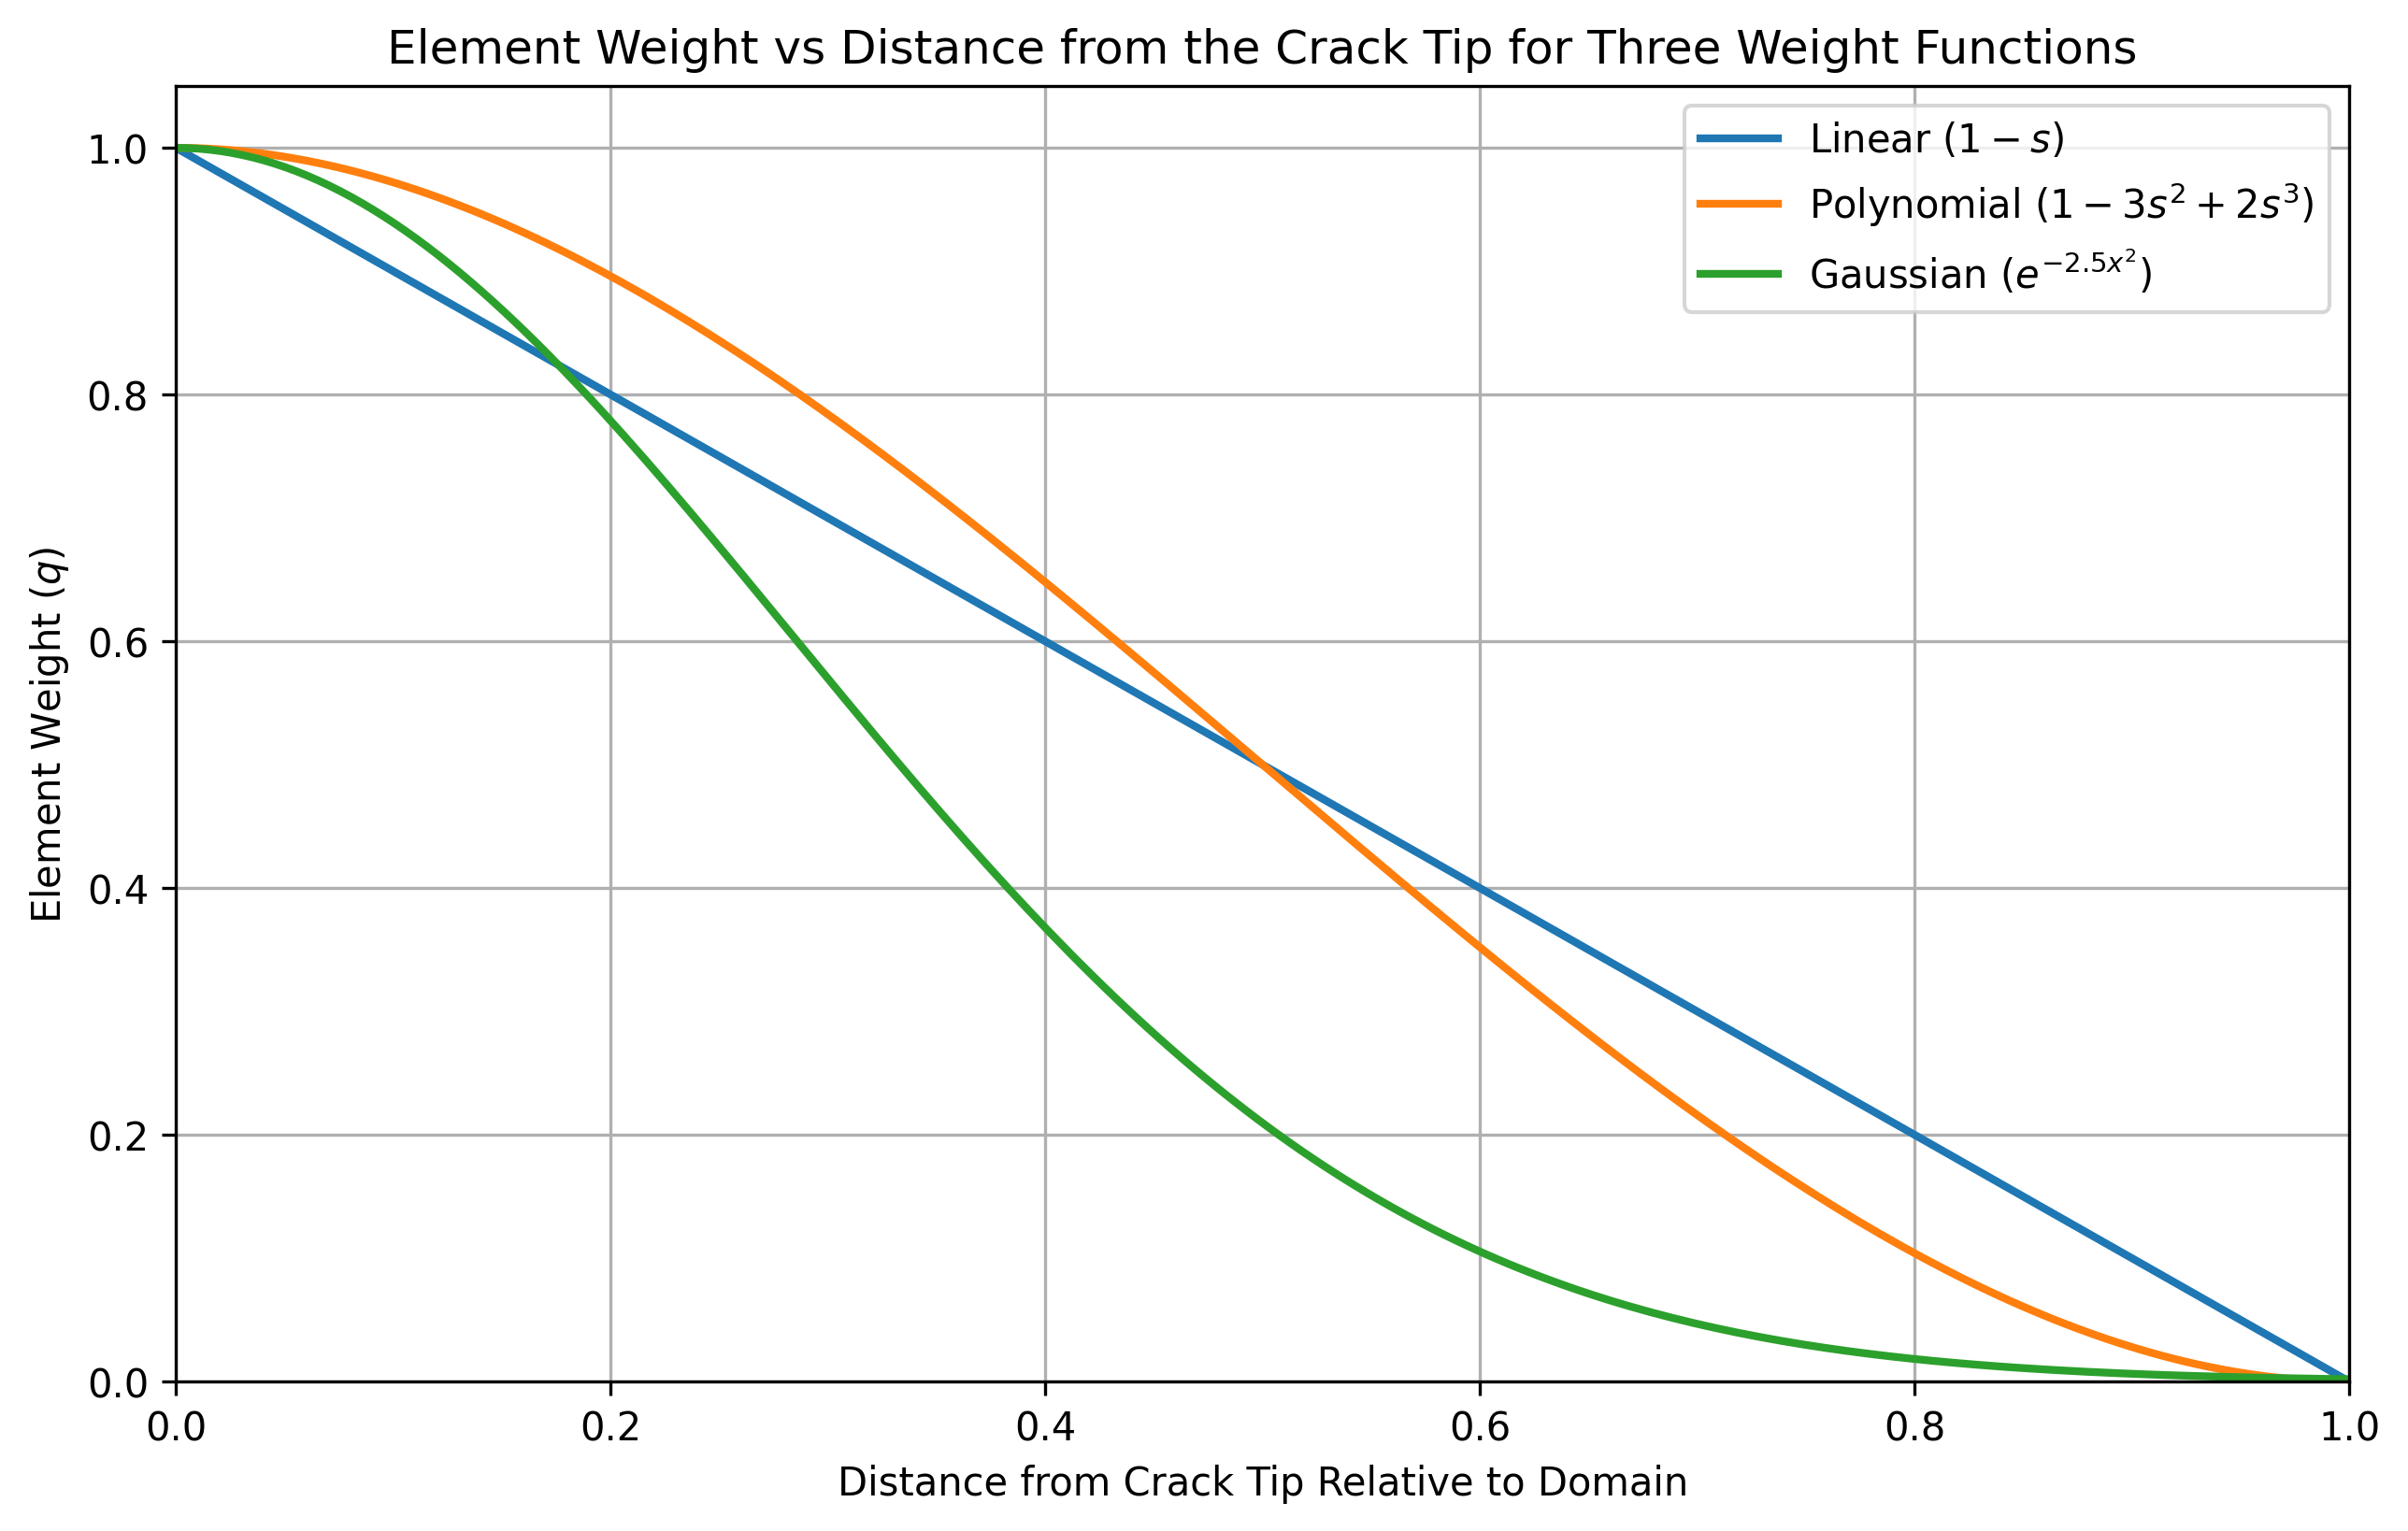
\includegraphics[width=\textwidth]{weight_function_comparison.png}
	\caption{Element weighting vs the distance of the element from the crack tip -- relative to the domain -- for the three weight functions investigated.}
	\label{fig:weight_function_comparison}
\end{figure}

 The linear weight function naturally exhibited a steady decrease of element weight along with the distance through the integration domain, and acted as the base of comparison for the other weight functions. The polynomial weight function placed the highest weighting on integration points close to the crack tip compared to the other weight functions, before intersecting the linear weight function at a relative distance of 0.5 before exhibiting a weights between those of the linear and Gaussian weight functions for integration points with relative distances of between 0.5 and 1. The Gaussian weight function placed a relatively high emphasis on the integration points close to the crack tip, before decaying very quickly and specifying element weights below those of the linear and polynomial weight functions for relative distances above around 0.2.
 
 The J-integral obtained using each weight function for the reference configuration was then again plotted against the integration domain, for both the 2D and 3D models -- this is presented in Figure \ref{fig:j_integral_vs_weight}. All of the three weight functions showed good agreement with each other beyond the first domain, with minimal variation being observed between each weight function for the 3D model. The linear and Gaussian weight functions for the 2D model exhibited some variation at the outer domains (between domains 6 and 10), while those same weight functions exhibited better agreement for the 3D model. This was likely due to numerical fluctuations, as the deviance did not exhibit a bias towards errors above or below the mean, and the errors between the linear and Gaussian weight functions were also different.

\begin{figure}[H]
	\centering
	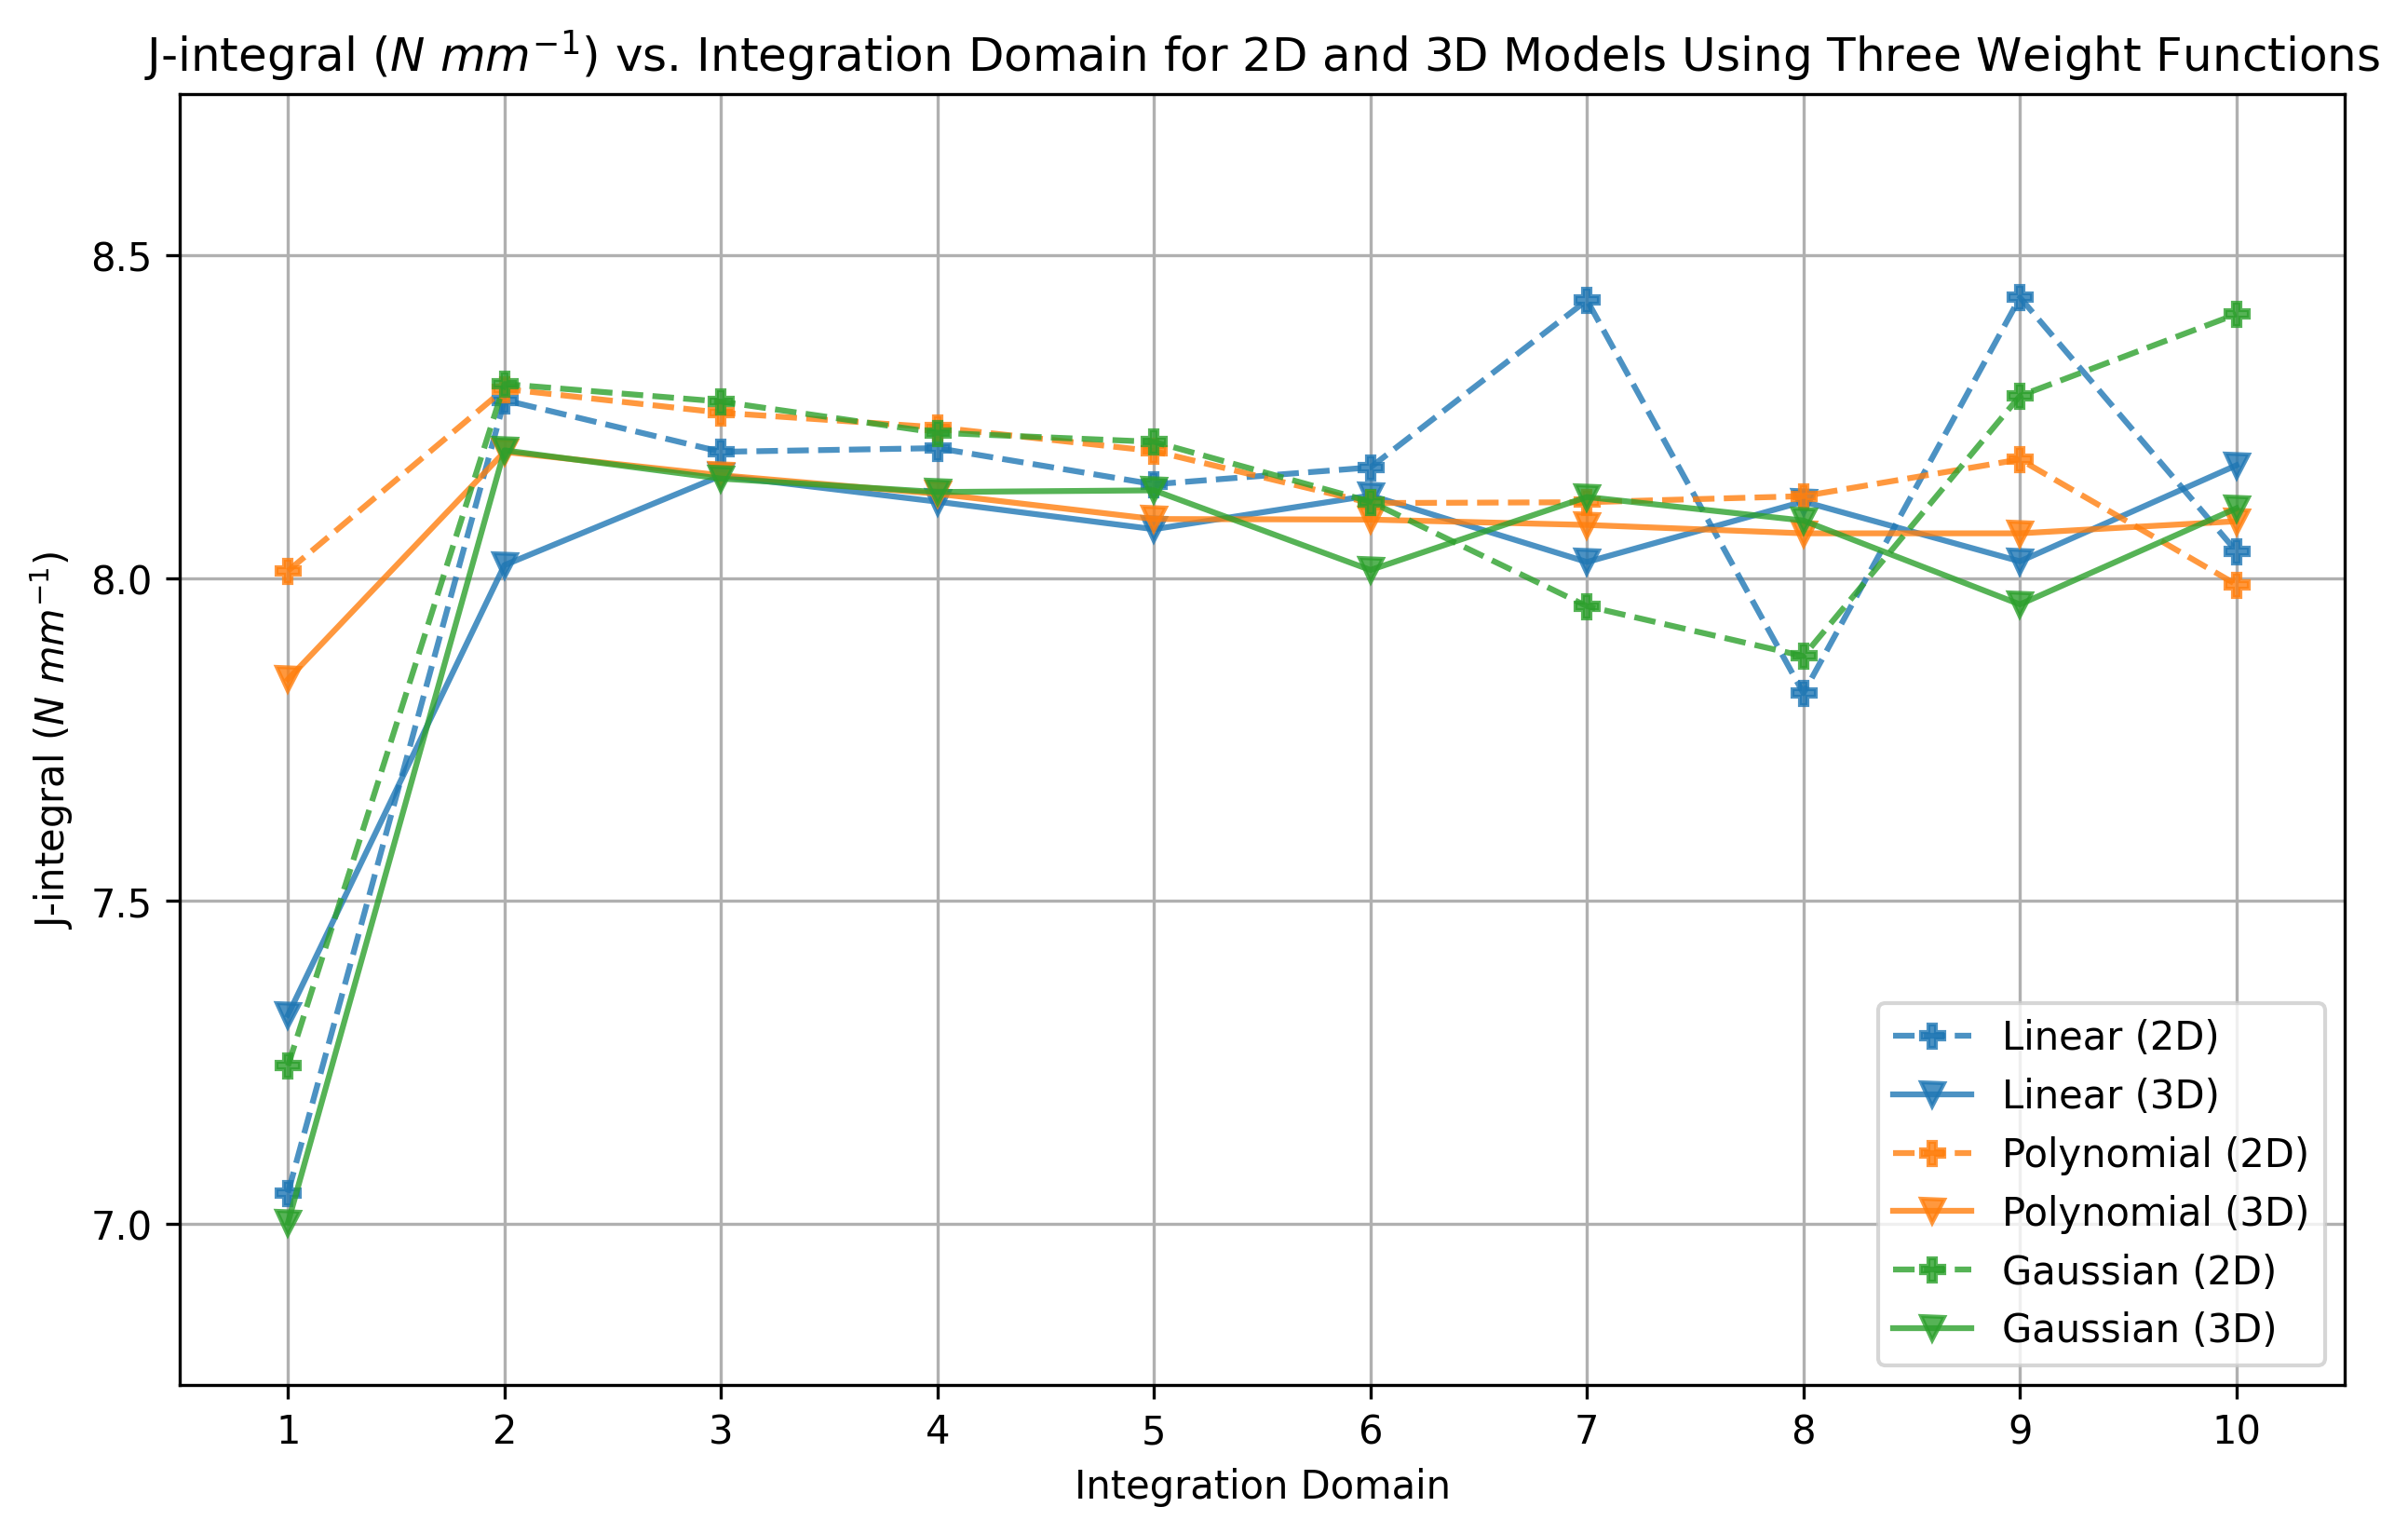
\includegraphics[width=\textwidth]{j_integral_vs_weight.png}
	\caption{Element weighting vs the distance of the element from the crack tip -- relative to the domain -- for the three weight functions investigated.}
	\label{fig:j_integral_vs_weight}
\end{figure}

The main difference between the weight functions was exhibited in the first domain, where the polynomial weight function produced J-integrals close to the analytical value of around 8.2, while the linear and Gaussian weight functions produced significantly lower J-integrals of between 7 and 7.5. This signified that the linear and Gaussian weight functions were potentially underestimating the contributions of the crack tip elements within the first domain. As the polynomial weight function decayed the most slowly of the three weight functions, it would have therefore placed the highest weights on the crack tip elements within the first domain. This increased weighting of the inner elements likely had a lesser impact within domains 2-10, but had a significant contribution within the first domain, which would have been dominated by the effects of the crack tip elements.

The polynomial weight function also showed the greatest amount of agreement between the 2D and 3D models - with the J-integral values showing close agreement for every domain. This was not the case for the linear and Gaussian weight functions, which exhibited somewhat significant disagreements between the results for the 2D and 3D models, for the outer domains. As the polynomial weight function produced the most domain-independent results while simultaneously exhibiting the closest agreement between the 2D and 3D models, it was selected as the most suitable weight function to perform the rest of the analysis. Although additional validation would be necessary to fully demonstrate the superiority of the polynomial weight function (for example, testing it against multiple crack lengths and configurations), the validation performed was considered to be satisfactory for this application.

\section{Crack Length}

Finally, once the mesh density, domains, and weight functions had been validated, the impact of the crack length on the J-integral and the stress intensity factor was investigated. Equation \ref{eq:j-integral_sif} demonstrates that the J-integral is proportional to the square of the stress intensity factor, while Equation \ref{eq:sif} demonstrates that the stress intensity factor is proportional to the square root of the crack length. Therefore, assuming a constant shape factor $B_i$, it would be expected that the stress intensity factor would exhibit a linear relationship with the crack length, while the J-integral would exhibit a second-degree polynomial relationship with the crack length. However, for the specific edge-crack configuration analysed, the shape factor exhibited a non-linear relationship with the crack length. Taking Equation \ref{eq:beta_edge_crack} and plotting it between a crack length of 0 mm and 25 mm for a plate with a constant width of 50 mm demonstrates the relationship between the crack length and the shape factor $\beta_{i}$, which is presented in Figure \ref{fig:shape_factor}.

\begin{figure}[H]
	\centering
	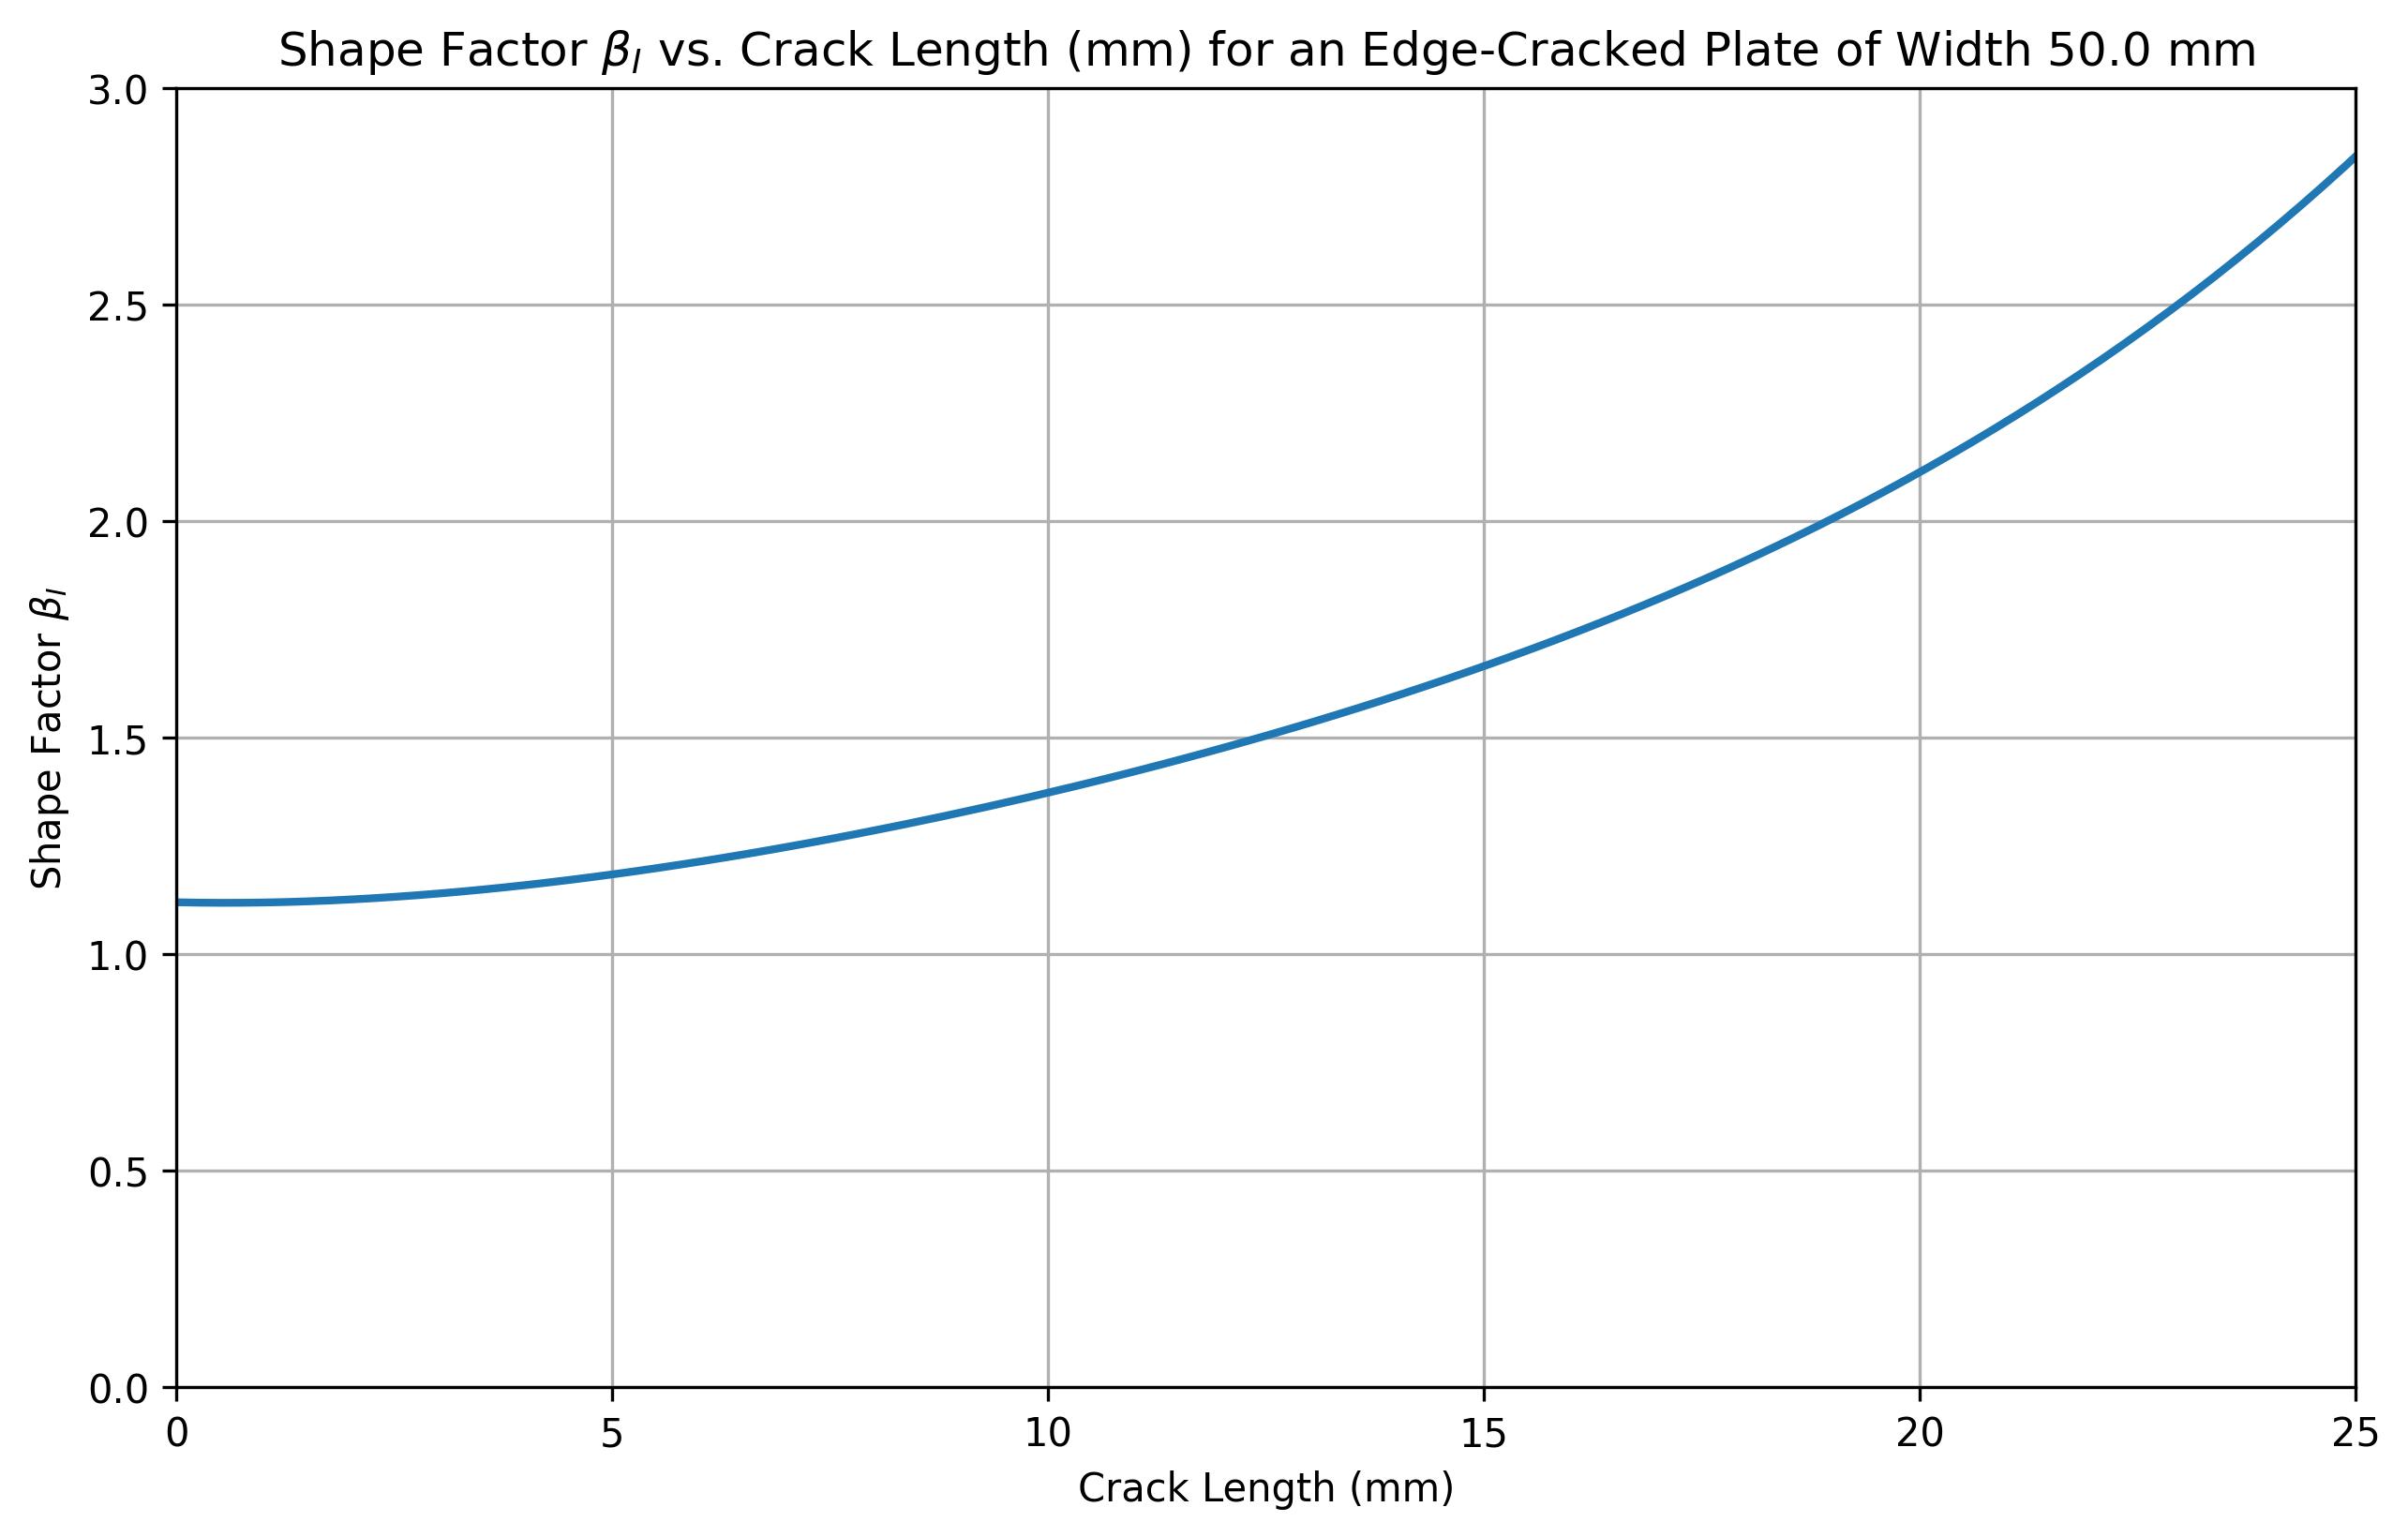
\includegraphics[width=\textwidth]{shape_factor.png}
	\caption{Shape Factor ($\beta_{i}$) vs Crack Length ($mm$) for an Edge-Cracked Plate with a Width of 50 mm.}
	\label{fig:shape_factor}
\end{figure}

Figure \ref{fig:shape_factor} clearly demonstrates that the shape factor $\beta_{i}$ increases as the crack length increases (and therefore the ratio of the crack length to the plate width $\frac{a}{b}$ also increases). This is because as the crack grows longer, there is a smaller remaining ligament (un-cracked plate ahead of the crack tip) to carry the load -- as the plate is of a finite width. Therefore, there is less material available to carry the remote tensile stress applied to the plate, and the influence of the free surface ahead of the crack becomes increasingly more significant \cite{anderson_fracture_2017}. As the stress intensity factor is directly proportional to $\beta_{i}$, it would therefore be expected that the relationship between the J-integral and the crack length, and the stress intensity factor and the crack length, would be of a higher-order than would be expected for a centre-cracked plate. It can also be observed that the plotted line crosses the y-axis at a value of 1.12 -- this is the shape factor for the special case of an edge crack in a semi-infinite body, where the shape factor remains constant regardless of the crack length due to the infinite ligament available ahead of the crack tip \cite{yuan_research_2023}.

A comparison was then performed between the J-integral results obtained from the outputs generated by the software for the 2D and 3D models, and the analytically obtained values -- using crack lengths between 2 mm and 25 mm. This is presented in Figure \ref{fig:j_integral_vs_crack_length}, which demonstrates the expected relationship between the J-integral and the crack length -- with the J-integral increasing as the crack length increases. The J-integral displayed a non-linear relationship with the crack length, with a polynomial of degree 4 showing a close fit with the plotted data. This was expected, due to the influence of the shape factor on the stress intensity factor, and therefore the J-integral. The inclusion of higher-order terms within the equation for the shape factor meant that the J-integral was expected to rise more quickly for this edge crack study, versus a configuration using a shape factor that did not change along with the crack length.

\begin{figure}[H]
	\centering
	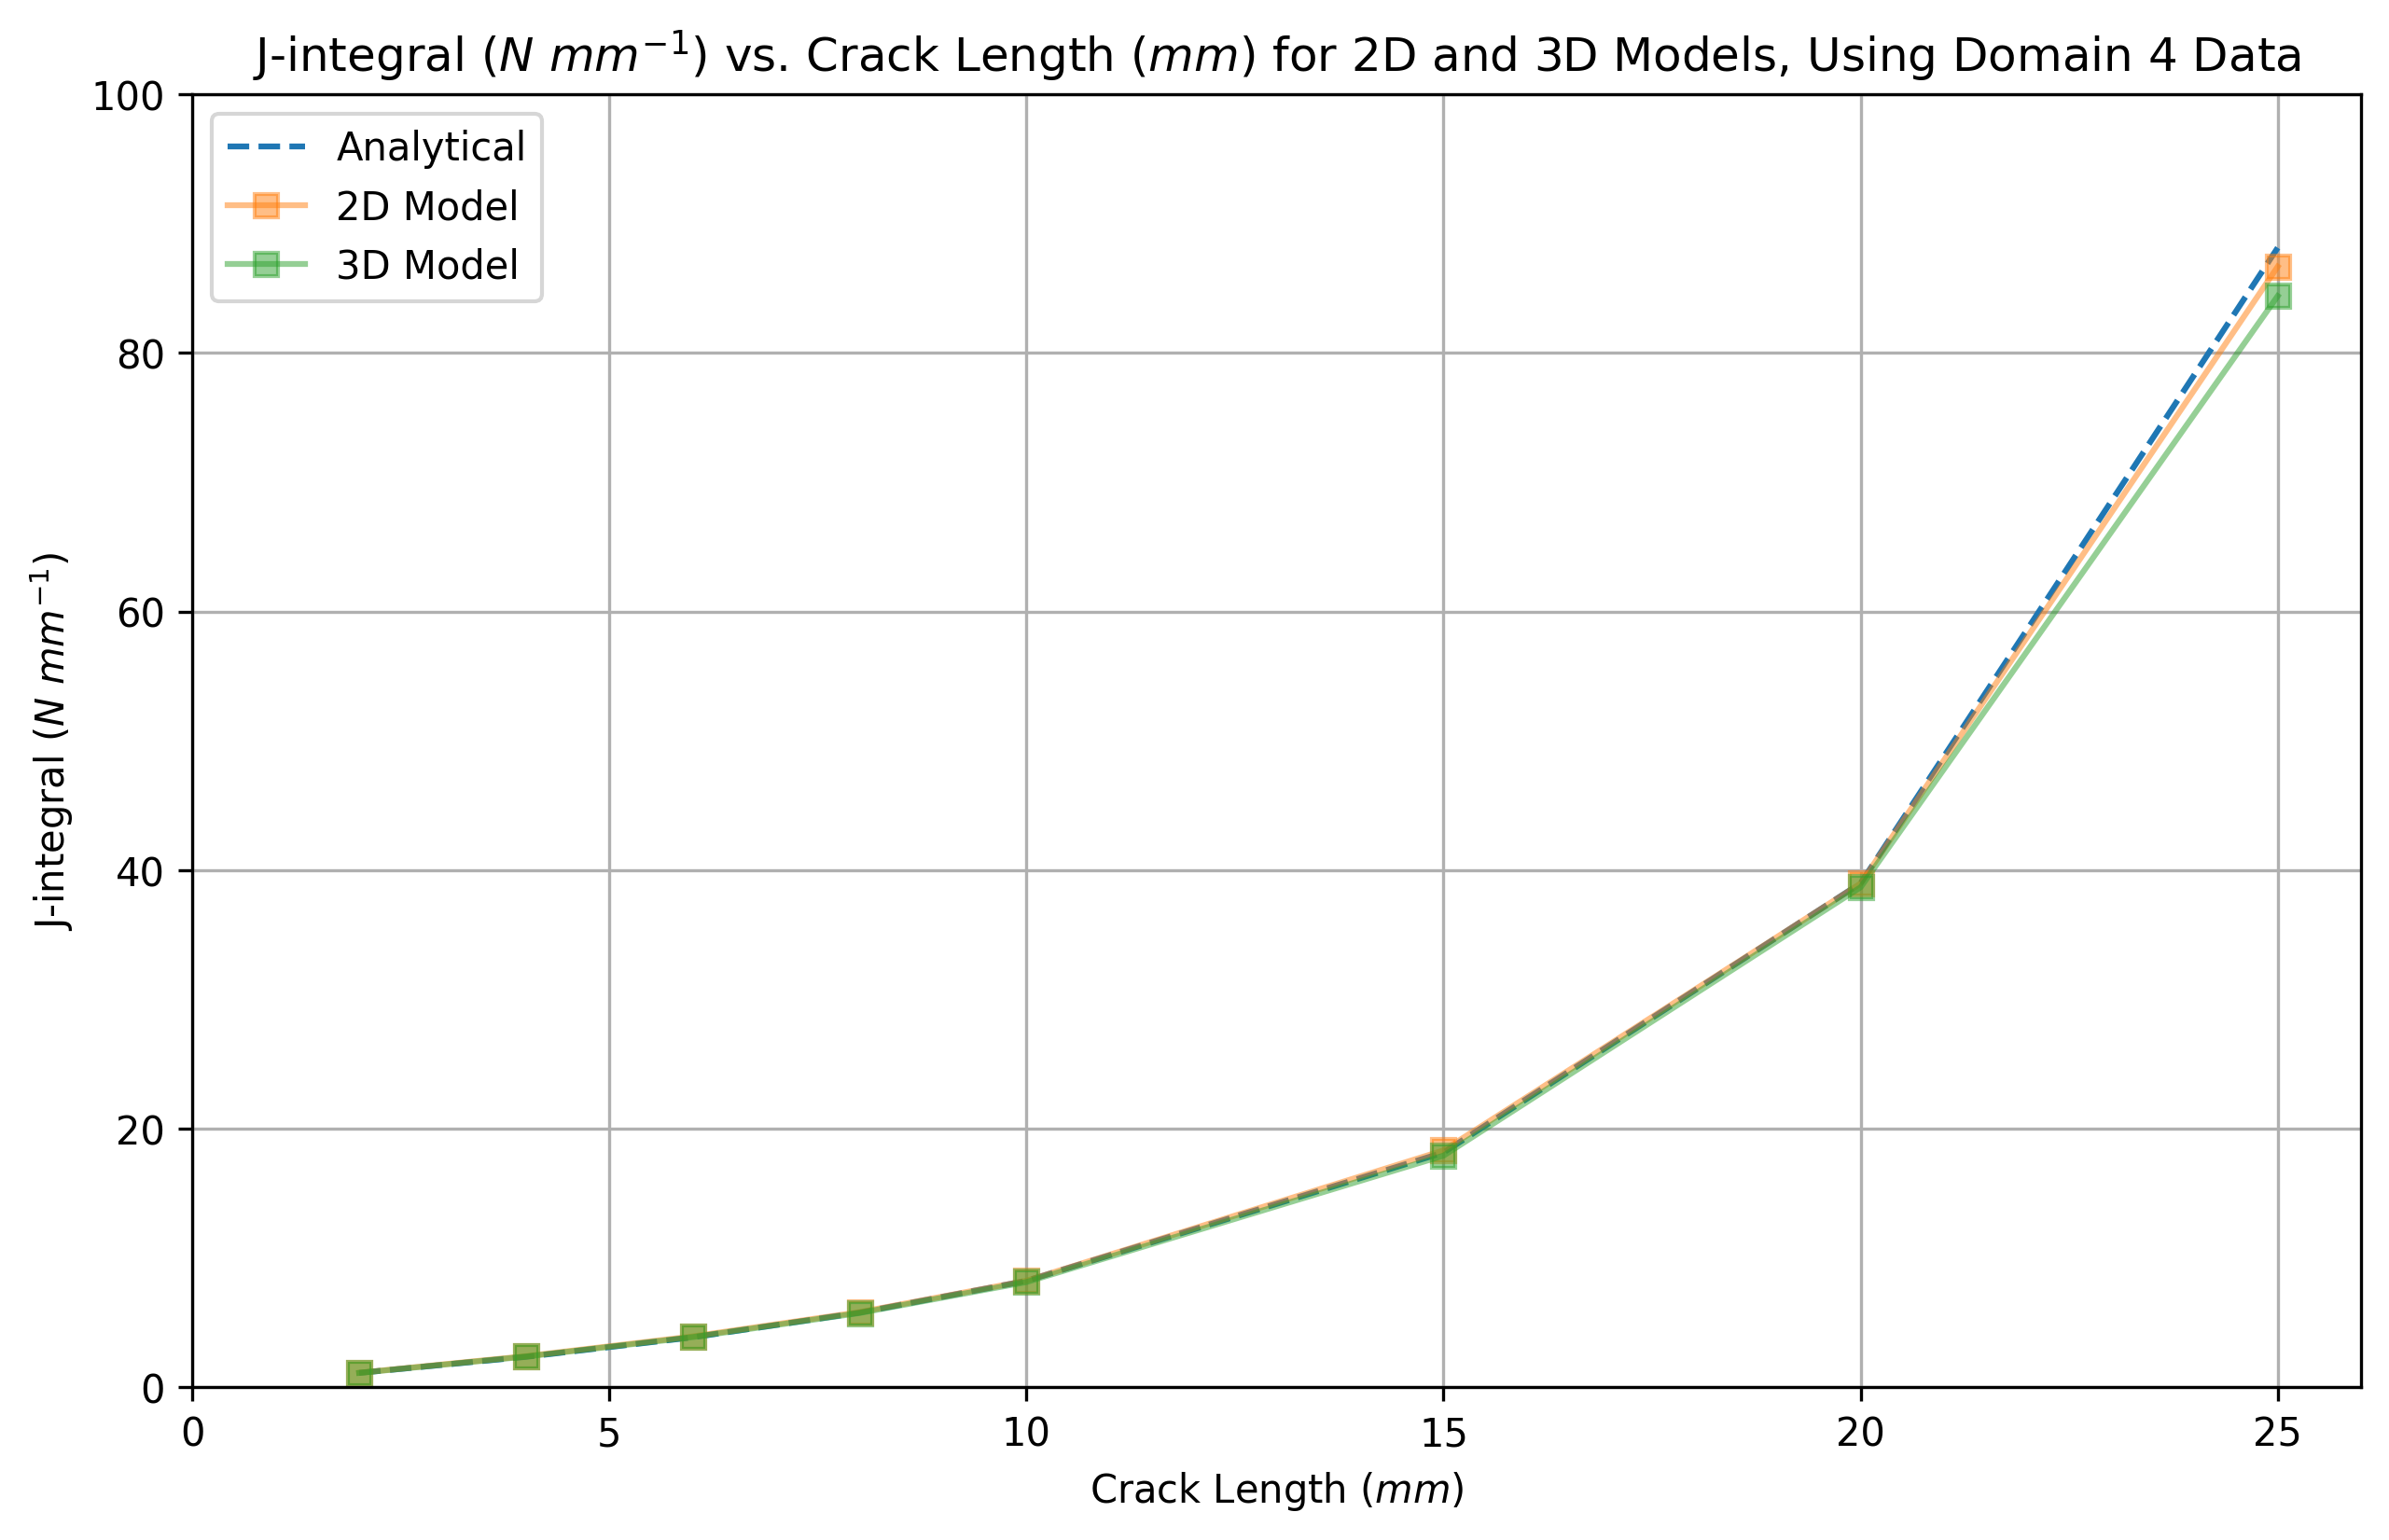
\includegraphics[width=\textwidth]{j_integral_vs_crack_length.png}
	\caption{J-integral ($N mm^{-1}$) vs crack length ($mm$) for 2D and 3D models using data from domain 4 and a polynomial weight function, compared to analytically calculated values.}
	\label{fig:j_integral_vs_crack_length}
\end{figure}

The J-integral calculated using the software agreed extremely well with the data obtained via the analytical method, with errors on the order of 1-2\% -- this also compared well with error rates observed within the literature \cite{yuan_research_2023}. Errors on this order are generally expected when using finite element analysis, due to the approximate nature of the method and the potential for small numerical errors. The 2D and 3D models used for the case study also produced results which agreed extremely closely -- again with differences of around 1-2\%. This clearly demonstrated that the equivalent domain integral method was implemented correctly within the software, and also showed that the method was equally valid for CPS6 and C3D10 elements in the selected case study.

A similar graph was plotted to understand the relationship between the stress intensity factor and the crack length -- again for the 2D and 3D models along with the analytical results. This is presented in Figure \ref{fig:sif_vs_crack_length}. The relationship between the stress intensity factor and the crack length also exhibited a non-linear relationship, with the stress intensity factor rising with the crack length -- although at a slower rate than the J-integral. This was expected as the J-integral is calculated using the square root of the J-integral, and therefore it would be expected to show a lower-order relationship with the crack length when compared to the J-integral. Again, the results obtained using the 2D and 3D models compared very favourably to the analytically-obtained results, verifying that the software could be used to calculate sufficiently accurate stress intensity factors, and therefore validating that the software met its intended purpose outlined in §\ref{sec:aims_objectives}.

\begin{figure}[H]
	\centering
	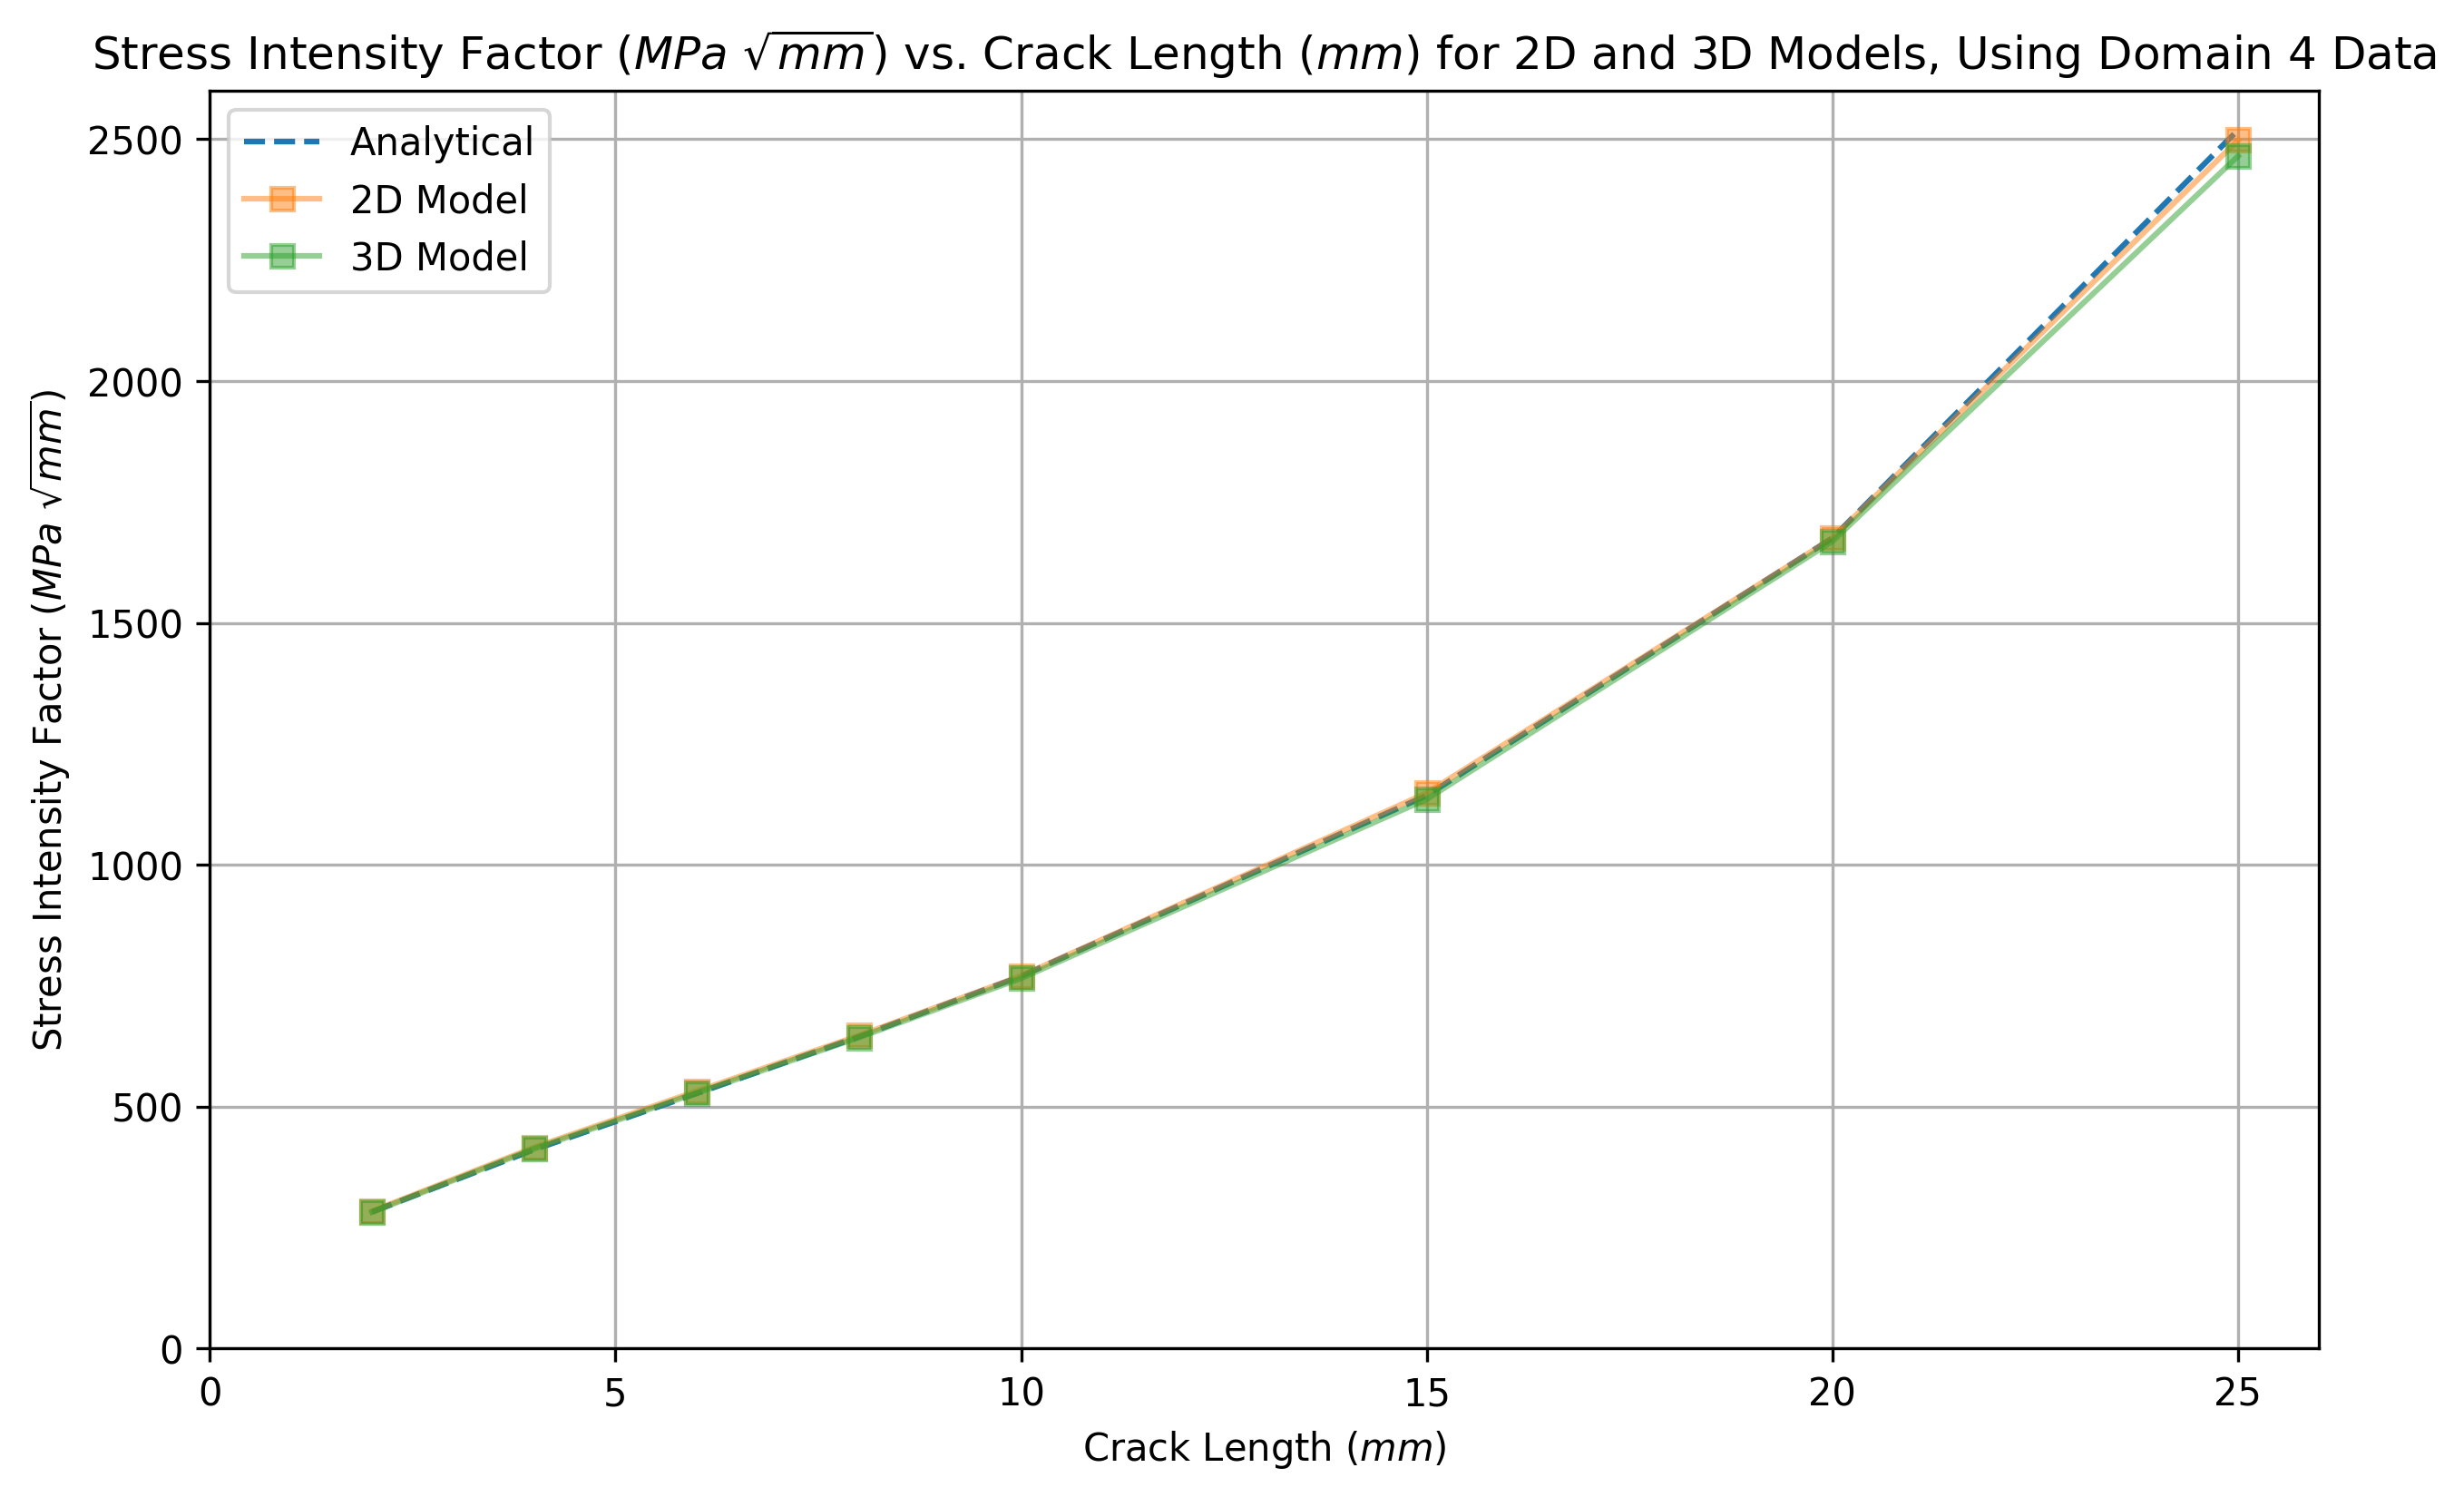
\includegraphics[width=\textwidth]{sif_vs_crack_length.png}
	\caption{Stress intensity factor ($MPa \sqrt{mm}$) vs crack length ($mm$) for 2D and 3D models using data from domain 4 and a polynomial weight function, compared to analytically obtained values.}
	\label{fig:sif_vs_crack_length}
\end{figure}

\newpage
For completeness, the stress intensity factors were recorded for each crack length, for both the 2D and 3D models. These are presented in Table \ref{tab:j_integral_comparison}.

\begin{table}[H]
	\caption{Comparison of J-integral values for various crack lengths: 2D vs. 3D FEA vs.\ analytical solution, with percentage error.}
	\centering
	\begin{tabular}{|r l|c|c|c|c|c|c|}
		\hline
		Crack Length & $mm$ & 2 & 6 & 10 & 15 & 20 & 25 \\ \hline
		Analytical SIF & $MPa \sqrt{mm}$ & 282.4  & 527.0  & 769.6  & 1143.2 & 1675.3 & 2519.1 \\
		2D SIF & $MPa \sqrt{mm}$ & 283.7  & 531.8  & 767.0  & 1148.3 & 1676.9 & 2498.1 \\
		2D Error & \% & +0.47 & +0.90 & +0.05 & +0.83 & +0.45 & -0.02 \\
		3D SIF & $MPa \sqrt{mm}$   & 281.7  & 528.2  & 765.1  & 1135.6 & 1668.6 & 2465.1 \\
		3D Error & \% & -0.22 & +0.23 & -0.58 & -0.66 & +0.40 & -2.14 \\ \hline
	\end{tabular}
	\label{tab:j_integral_comparison}
\end{table}


